\section{Akteursübersicht}
\begin{tabularx}{\textwidth}{ p{.2\textwidth} | p{.2\textwidth} | X }
	\multicolumn{3}{>{\hsize=\dimexpr2\hsize+2\tabcolsep+\arrayrulewidth\relax}X}{\centering \textbf{Beschreibung der Akteure}} \\
	\multicolumn{3}{X}{\vspace{1cm}} \\
	\textbf{Akteur} & \textbf{Beschreibung} & \textbf{Verwendet in Anwendungsfall} \\ \hline
	Spielleiter:innen & Spielleiter:innen erstellen und verwalten Planspiele & Lehrer-Registrierungs-URL erstellen, Planspiel erstellen, Planspiel beenden, Import von Planspielen, Export von Planspielen, Alle Bestellungen einsehen \\ \hline
	Lehrkräfte & Lehrkräfte erstellen und verwalten landeseigene Großhändler & Lehrkraft-Registrierung via Deeplink, SuS-Deeplink erstellen, Großhändler hinzufügen, Großhändler löschen, Import von Grosshändlern oder Produkten, Export von Grosshändlern oder Produkten, Produkte hinzufügen, Produkte löschen, Kategorien hinzufügen, Kategorien bearbeiten, Kategorien löschen, Bestellungen verwalten, Lehrkraft/SuS-Login, Fehlermeldung, Passwort zurücksetzen \\ \hline
	SuS-Unternehmen & Sus-Unternehmen bestellen Produkte bei Großhändlern &  Großhändlerliste ansehen via Deeplink, SuS-Registrierung bei Großhändler, Bestellungen einsehen, Produkt in den Warenkorb hinzufügen, Produkt aus dem Warenkorb entfernen, Bestellen, Lehrkraft/SuS-Login, Fehlermeldung, Passwort zurücksetzen \\ \hline
\end{tabularx}
\label{fig:akteur-tabelle}

\newpage
\section{Mockups der Funktionalität}

Ein Bild über die Funktionalität der Software kann man sich über unsere Interaktiven Mockups machen.

Mockup der Weboberfläche aus Lehrersicht: \href{https://www.figma.com/proto/J6wDnjPfZRockWqW8Hru8f/Untitled?page-id=0%3A1&type=design&node-id=85-3641&viewport=561%2C-131%2C0.15&t=UGccSvhlxAx3oc3p-1&scaling=contain&starting-point-node-id=85%3A3641&mode=design}{Lehrersicht Mockup}

Mockup der Weboberfläche aus SuS-Unternehmens-Sicht: \href{https://www.figma.com/proto/J6wDnjPfZRockWqW8Hru8f/Untitled?page-id=85%3A2840&type=design&node-id=85-3174&viewport=920%2C336%2C0.14&t=vbKEeDjeuEgnx2sG-1&scaling=min-zoom&starting-point-node-id=85%3A3174}{SuS-Unternehmen-Sicht Mockup}

Mockup der Android-App für SuS-Unternehmer: \href{https://www.figma.com/proto/J6wDnjPfZRockWqW8Hru8f/Untitled?page-id=78%3A2348&type=design&node-id=78-2592&viewport=685%2C411%2C0.35&t=vrfZ5igwusJ8psCc-1&scaling=min-zoom&starting-point-node-id=78%3A2592}{SuS-Unternehmer Android-App Mockup}

\bigskip
Das Entsprechen der entwickelten Software zu diesen Mockups ist nicht bindend, sondern sie dienen nur für ein intuitiveres Verständnis des Aufbaus der Software. In \ref{af-tabellen} folgen detailliertere, tabellarische Beschreibungen zur Funktionsweise der Software, welche wir auch als bindend betrachten.

\section{Anwendungsfalldiagramm}
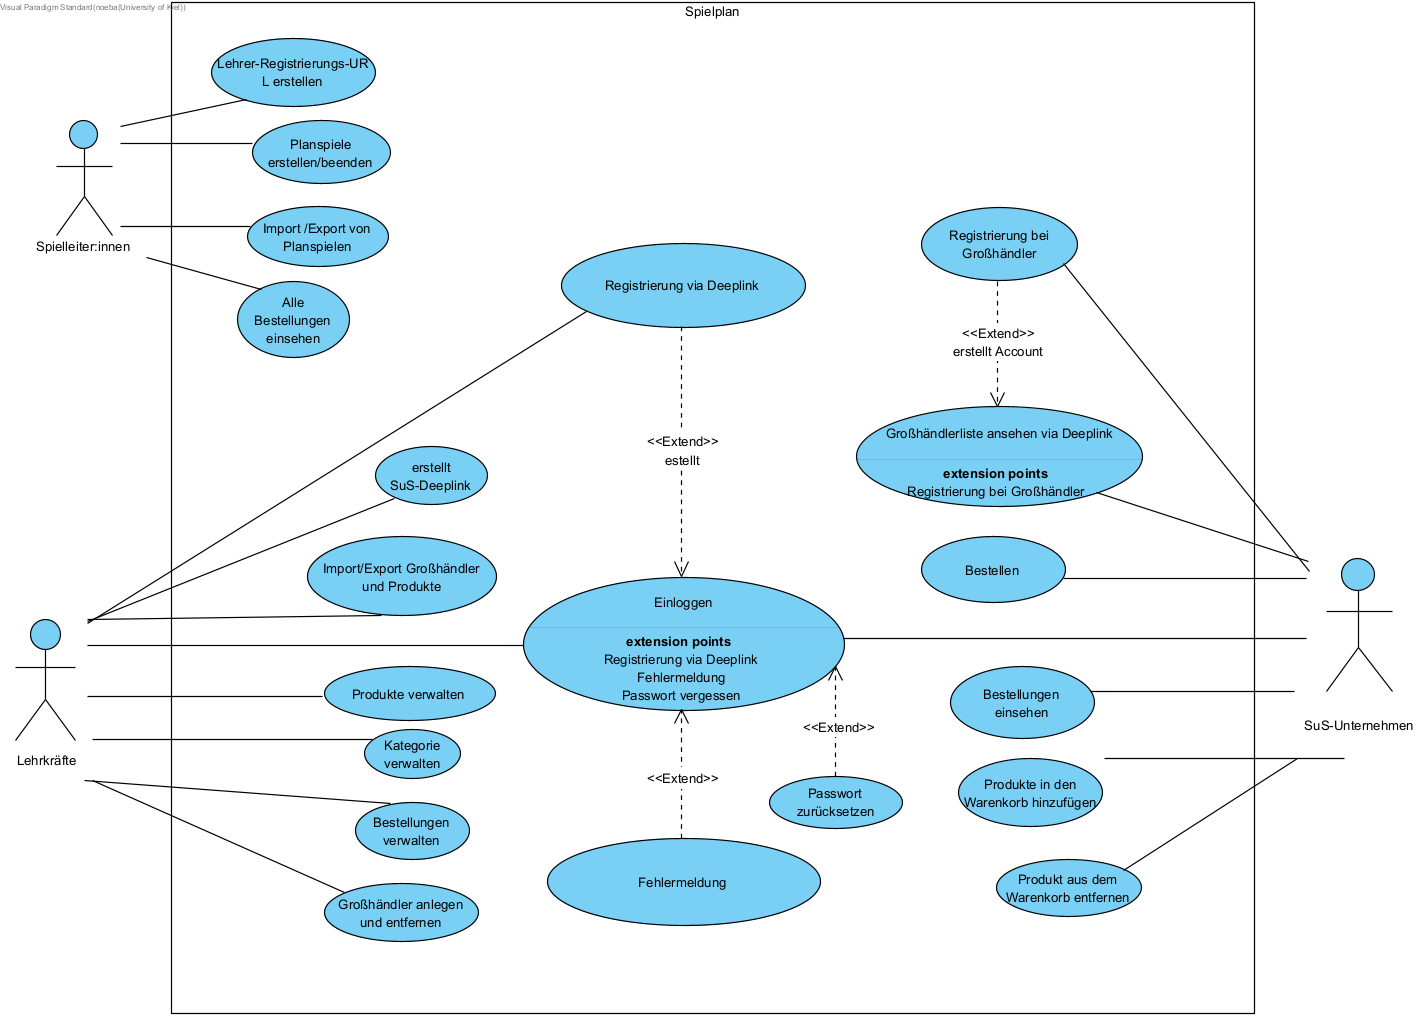
\includegraphics[width=\textwidth,height=0.65\textheight]{img/Planspiel}

\section{Anwendungsfälle in Tabellarischer Form} \label{af-tabellen}
\subsection{Anwendungsfälle von Spielleitern}

% Lehrer Deeplink erstellen
\begin{tabularx}{\textwidth}{ X | X }
	\multicolumn{2}{>{\hsize=\dimexpr2\hsize+2\tabcolsep+\arrayrulewidth\relax}X}{\centering \textbf{Lehrer-Registrierungs-URL erstellen}} \\
	\multicolumn{2}{X}{\vspace{1cm}} \\
	\textbf{Anwendungsfall ID} & ULE \\ \hline
	\textbf{Anwendungsfallname} & Lehrer-Registrierungs-URL erstellen \\ \hline
	\textbf{Initiierender Akteur} & Spielleiter \\ \hline
	\textbf{Weitere Akteure} & Lehrkraft \\ \hline
	\textbf{Kurzbeschreibung} & Der Spielleiter erstellt eine URL, die es der Lehrkraft ermöglicht, sich im System zu registrieren. \\ \hline
	\textbf{Vorbedingungen} & Der Spielleiter hat eine Befehlszeile auf dem Server offen und mindestens ein Planspiel läuft. \\ \hline
	\textbf{Nachbedingungen} & Eine URL wurde erstellt und der Lehrkraft zur Verfügung gestellt, die diesen für die Regristrierung nutzt. \\ \hline
	\textbf{Ablauf} &
		\begin{enumerate}
			\item Der Spielleiter gibt den entsprechenden Befehl ein.
			\item Eine entsprechende URL, die für das einzige aktuell laufende Planspiel gültig ist, wird ausgegeben.
			\item Der Spielleiter stellt die URL der Lehrkraft bereit.
		\end{enumerate} \\ \hline
	\textbf{Alternative} &
		\begin{enumerate}
			\item Der Spielleiter gibt den entsprechenden Befehl ein.
			\item Der Spielleiter gibt in einer interaktiven Eingabe an, für welches der laufenden Planspiele die URL generiert werden soll.
			\item Eine entsprechende URL wird ausgegeben.
			\item Der Spielleiter stellt die URL der Lehrkraft bereit.
		\end{enumerate} \\ \hline
	\textbf{Ausnahme} & Der Spielleiter gibt ein Planspiel an, welches nicht existiert. \\ \hline
	\textbf{Benutzte Anwendungsfälle} & - \\ \hline
	\textbf{Spezielle Anforderungen} & - \\ \hline
	\textbf{Annahmen} & -
\end{tabularx}
\label{fig:anwendungsfall-ule}

% Planspiele verwalten

\begin{tabularx}{\textwidth}{ X | X }
	\multicolumn{2}{>{\hsize=\dimexpr2\hsize+2\tabcolsep+\arrayrulewidth\relax}X}{\centering \textbf{Planspiel erstellen}} \\
	\multicolumn{2}{X}{\vspace{1cm}} \\
	\textbf{Anwendungsfall ID} & PE \\ \hline
	\textbf{Anwendungsfallname} & Planspiel erstellen \\ \hline
	\textbf{Initiierender Akteur} & Spielleiter \\ \hline
	\textbf{Weitere Akteure} & - \\ \hline
	\textbf{Kurzbeschreibung} & Der Spielleiter erstellt und startet ein Planspiel. \\ \hline
	\textbf{Vorbedingungen} & - \\ \hline
	\textbf{Nachbedingungen} & Das Planspiel ist gestartet und läuft. \\ \hline
	\textbf{Ablauf} &
	\begin{enumerate}
			\item Spielleiter öffnet die Server Command line.
			\item Spielleiter gibt den Erstellungsbefehl ein.
		\end{enumerate} \\ \hline
	\textbf{Ausnahme} & - \\ \hline
	\textbf{Benutzte Anwendungsfälle} & - \\ \hline
	\textbf{Spezielle Anforderungen} & - \\ \hline
	\textbf{Annahmen} & -
\end{tabularx}
\label{fig:anwendungsfall-pe}

\begin{tabularx}{\textwidth}{ X | X }
	\multicolumn{2}{>{\hsize=\dimexpr2\hsize+2\tabcolsep+\arrayrulewidth\relax}X}{\centering \textbf{Planspiel beenden}} \\
	\multicolumn{2}{X}{\vspace{1cm}} \\
	\textbf{Anwendungsfall ID} & PLB \\ \hline
	\textbf{Anwendungsfallname} & Planspiel beenden \\ \hline
	\textbf{Initiierender Akteur} & Spielleiter \\ \hline
	\textbf{Weitere Akteure} & - \\ \hline
	\textbf{Kurzbeschreibung} & Der Spielleiter beendet ein Planspiel. \\ \hline
	\textbf{Vorbedingungen} & Das Planspiel läuft bereits. \\ \hline
	\textbf{Nachbedingungen} & Das Planspiel ist beendet und läuft nicht mehr. \\ \hline
	\textbf{Ablauf} &
		\begin{enumerate}
			\item Spielleiter öffnet Server Command line.
			\item Spielleiter gibt Beendungsbefehl ein.
		\end{enumerate} \\ \hline
	\textbf{Ausnahme} & - \\ \hline
	\textbf{Benutzte Anwendungsfälle} & - \\ \hline
	\textbf{Spezielle Anforderungen} & - \\ \hline
	\textbf{Annahmen} & -
\end{tabularx}
\label{fig:anwendungsfall-plb}

% Import/Export von Planspielen
\begin{tabularx}{\textwidth}{ X | X }
	\multicolumn{2}{>{\hsize=\dimexpr2\hsize+2\tabcolsep+\arrayrulewidth\relax}X}{\centering \textbf{Import von Planspielen}} \\
	\multicolumn{2}{X}{\vspace{1cm}} \\
	\textbf{Anwendungsfall ID} & IP \\ \hline
	\textbf{Anwendungsfallname} & Import von Planspielen \\ \hline
	\textbf{Initiierender Akteur} & Spielleiter \\ \hline
	\textbf{Weitere Akteure} & - \\ \hline
	\textbf{Kurzbeschreibung} & Der Spielleiter kann ganze Planspiele als JSON-Datei importieren. \\ \hline
	\textbf{Vorbedingungen} & Der Spielleiter hat ein Planspiel erstellt und ein exportiertes Planspiel liegt als JSON-Datei vor. \\ \hline
	\textbf{Nachbedingungen} & Der alte Spielstand wird vom importierten Spielstand überschrieben und kann genutzt werden. \\ \hline
	\textbf{Ablauf} &
		\begin{enumerate}
			\item Server Command line öffnen.
			\item Import-Command inklusive JSON-Datei eingeben.
			\item Command absenden.
		\end{enumerate} \\ \hline
	\textbf{Alternative} & - \\ \hline
	\textbf{Ausnahme} &
		\begin{enumerate}
			\item Server Command line öffnen.
			\item Import-Command inklusive JSON-Datei eingeben.
			\item Command absenden.
			\item Fehlermeldung wird angezeigt, dass ein falsches Dateiformat vorliegt.
		\end{enumerate} \\ \hline
\textbf{Benutzte Anwendungsfälle} & - \\ \hline
	\textbf{Spezielle Anforderungen} & - \\ \hline
	\textbf{Annahmen} & -
\end{tabularx}
\label{fig:anwendungsfall-ip}

\begin{tabularx}{\textwidth}{ X | X }
	\multicolumn{2}{>{\hsize=\dimexpr2\hsize+2\tabcolsep+\arrayrulewidth\relax}X}{\centering \textbf{Export von Planspielen}} \\
	\multicolumn{2}{X}{\vspace{1cm}} \\
	\textbf{Anwendungsfall ID} & EP \\ \hline
	\textbf{Anwendungsfallname} & Export von Planspielen \\ \hline
	\textbf{Initiierender Akteur} & Spielleiter \\ \hline
	\textbf{Weitere Akteure} & - \\ \hline
	\textbf{Kurzbeschreibung} & Der Spielleiter kann ganze Planspiele als JSON-Datei exportieren. \\ \hline
	\textbf{Vorbedingungen} & Es läuft bereits ein Planspiel vor. \\ \hline
	\textbf{Nachbedingungen} & In dem Ordner, wo der Befehl ausgeführt wurde, ist eine JSON-Datei, die das angegebene Planspiel repräsentiert. \\ \hline
	\textbf{Ablauf} &
		\begin{enumerate}
			\item Server Command line öffnen.
			\item Export-Command eingeben.
			\item Command absenden.
		\end{enumerate} \\ \hline
	\textbf{Alternative} & - \\ \hline
	\textbf{Ausnahme} & - \\ \hline
\textbf{Benutzte Anwendungsfälle} & - \\ \hline
	\textbf{Spezielle Anforderungen} & - \\ \hline
	\textbf{Annahmen} & -
\end{tabularx}
\label{fig:anwendungsfall-ep}

% alle Bestellungen verwalten
\begin{tabularx}{\textwidth}{ X | X }
	\multicolumn{2}{>{\hsize=\dimexpr2\hsize+2\tabcolsep+\arrayrulewidth\relax}X}{\centering \textbf{Alle Bestellungen einsehen}} \\
	\multicolumn{2}{X}{\vspace{1cm}} \\
	\textbf{Anwendungsfall ID} & ABE \\ \hline
	\textbf{Anwendungsfallname} & Alle Bestellungen einsehen \\ \hline
	\textbf{Initiierender Akteur} & Spielleiter \\ \hline
	\textbf{Weitere Akteure} & - \\ \hline
	\textbf{Kurzbeschreibung} & Der Spielleiter sieht eine Liste an Bestellungen aus allen Ländern ein. \\ \hline
	\textbf{Vorbedingungen} & Das Spiel läuft. \\ \hline
	\textbf{Nachbedingungen} & Der Spielleiter bekommt in der Commandline alle Bestellungen (d.h. welches Planspiel, Großhändler, Produkt, Kunde, Stückzahl) in Textform ausgegeben. \\ \hline
	\textbf{Ablauf} &
		\begin{enumerate}
			\item Server Command line öffnen.
			\item Befehl zum Ausgeben aller Bestellungen eingeben.
		\end{enumerate} \\ \hline
	\textbf{Alternative} & - \\ \hline
	\textbf{Ausnahme} & - \\ \hline
	\textbf{Benutzte Anwendungsfälle} & - \\ \hline
	\textbf{Spezielle Anforderungen} & - \\ \hline
	\textbf{Annahmen} & -
\end{tabularx}
\label{fig:anwendungsfall-abe}

\subsection{Anwendungsfälle für Lehrkräfte}
% Registrierung via Deeplink

\begin{tabularx}{\textwidth}{ X | X }
	\multicolumn{2}{>{\hsize=\dimexpr2\hsize+2\tabcolsep+\arrayrulewidth\relax}X}{\centering \textbf{Lehrkraft-Registrierung via Deeplink}} \\
	\multicolumn{2}{X}{\vspace{1cm}} \\
	\textbf{Anwendungsfall ID} & RGL \\ \hline
	\textbf{Anwendungsfallname} & Lehrkraft-Registrierung via Deeplink \\ \hline
	\textbf{Initiierender Akteur} & Lehrkraft \\ \hline
	\textbf{Weitere Akteure} & Spielleiter:innen \\ \hline
	\textbf{Kurzbeschreibung} & Lehrkraft registriert sich anhand einer URL. \\ \hline
	\textbf{Vorbedingungen} & Spielleiter:innen hat eine URL erstellt. \\ \hline
	\textbf{Nachbedingungen} & Der Account ist erstellt und man könnte sich erfolgreich einloggen. \\ \hline
	\textbf{Ablauf} &
		\begin{enumerate}
			\item Lehrkraft bekommt eine URL vom Spielleiter:innen.
			\item Lehrkraft öffnet URL.
			\item Lehrkraft trägt Registrierungsdaten (Name, E-Mail, Land und Passwort) in das Formular ein.
			\item Lehrkraft bestätigt Daten per Klick auf Schaltfläche.
		\end{enumerate} \\ \hline
	\textbf{Alternative} & - \\ \hline
	\textbf{Ausnahme} & - \\ \hline
	\textbf{Benutzte Anwendungsfälle} & - \\ \hline
	\textbf{Spezielle Anforderungen} & - \\ \hline
	\textbf{Annahmen} & -
\end{tabularx}
\label{fig:anwendungsfall-rgl}

% SuS-Deeplink erstellen

\begin{tabularx}{\textwidth}{ X | X }
	\multicolumn{2}{>{\hsize=\dimexpr2\hsize+2\tabcolsep+\arrayrulewidth\relax}X}{\centering \textbf{SuS-Deeplink erstellen}} \\
	\multicolumn{2}{X}{\vspace{1cm}} \\
	\textbf{Anwendungsfall ID} & DES \\ \hline
	\textbf{Anwendungsfallname} & SuS-Deeplink erstellen \\ \hline
	\textbf{Initiierender Akteur} & Lehrkraft \\ \hline
	\textbf{Weitere Akteure} & SuS-Unternehmen \\ \hline
	\textbf{Kurzbeschreibung} & Die Lehrkraft erstellt eine URL, über die sich SuS-Unternehmen die landeseigenen Großhändler ansehen und dort registrieren können. \\ \hline
	\textbf{Vorbedingungen} & Die Lehrkraft ist eingeloggt. \\ \hline
	\textbf{Nachbedingungen} & Die Lehrkraft bekommt eine URL mit den beschriebenen Eigenschaften ausgegeben. \\ \hline
	\textbf{Ablauf} &
		\begin{enumerate}
			\item Die Lehrkraft navigiert zu der \glqq Registrierungslink erstellen\grqq-Oberfläche.
			\item Die URL wird generiert.
			\item Die URL wird der Lehrkraft bereitgestellt.
		\end{enumerate} \\ \hline
	\textbf{Alternative} & - \\ \hline
	\textbf{Ausnahme} & - \\ \hline
	\textbf{Benutzte Anwendungsfälle} & - \\ \hline
	\textbf{Spezielle Anforderungen} & - \\ \hline
	\textbf{Annahmen} & -
\end{tabularx}
\label{fig:anwendungsfall-des}

% Großhändler hinzufügen
\begin{tabularx}{\textwidth}{ X | X }
	\multicolumn{2}{>{\hsize=\dimexpr2\hsize+2\tabcolsep+\arrayrulewidth\relax}X}{\centering \textbf{Großhändler hinzufügen}} \\
	\multicolumn{2}{X}{\vspace{1cm}} \\
	\textbf{Anwendungsfall ID} & GH \\ \hline
	\textbf{Anwendungsfallname} & Großhändler hinzufügen \\ \hline
	\textbf{Initiierender Akteur} & Lehrkraft \\ \hline
	\textbf{Weitere Akteure} & - \\ \hline
	\textbf{Kurzbeschreibung} & Die Lehrkraft fügt einen Großhändler zum Spiel hinzu. \\ \hline
	\textbf{Vorbedingungen} & Die Lehrkraft ist im System angemeldet. \\ \hline
	\textbf{Nachbedingungen} & Ein neuer Großhändler wurde zum System hinzugefügt und ist der Liste sichtbar. \\ \hline
	\textbf{Ablauf} &
	\begin{enumerate}
		\item Die Lehrkraft navigiert zur Großhändlerverwaltung.
		\item Das Spiel bestätigt die Hinzufügung des Großhändlers mit dem eingegebenem Namen.
	\end{enumerate} \\ \hline
	\textbf{Alternative} & - \\ \hline
	\textbf{Ausnahme} & - \\ \hline
	\textbf{Benutzte Anwendungsfälle} & - \\ \hline
	\textbf{Spezielle Anforderungen} & - \\ \hline
	\textbf{Annahmen} & - \\ \hline
\end{tabularx}
\label{fig:anwendungsfall-gh}

% Großhändler löschen
\begin{tabularx}{\textwidth}{ X | X }
	\multicolumn{2}{>{\hsize=\dimexpr2\hsize+2\tabcolsep+\arrayrulewidth\relax}X}{\centering \textbf{Großhändler löschen}} \\
	\multicolumn{2}{X}{\vspace{1cm}} \\
	\textbf{Anwendungsfall ID} & GL \\ \hline
	\textbf{Anwendungsfallname} & Großhändler löschen \\ \hline
	\textbf{Initiierender Akteur} & Lehrkraft \\ \hline
	\textbf{Weitere Akteure} & - \\ \hline
	\textbf{Kurzbeschreibung} & Die Lehrkraft entfernt einen Großhändler aus dem Spiel. \\ \hline
	\textbf{Vorbedingungen} & Die Lehrkraft ist im System angemeldet und der zu löschende Großhändler ist bereits im Spiel vorhanden. \\ \hline
	\textbf{Nachbedingungen} & Der Großhändler wurde aus dem System entfernt und ist nicht mehr in der Liste sichtbar. \\ \hline
	\textbf{Ablauf} &
	\begin{enumerate}
		\item Die Lehrkraft navigiert zur Großhändlerverwaltung.
		\item Die Lehrkraft wählt den zu löschenden Großhändler aus.
		\item Der Großhändler ist nicht mehr in der Liste zu finden.
	\end{enumerate} \\ \hline
	\textbf{Alternative} & - \\ \hline
	\textbf{Ausnahme} & - \\ \hline
	\textbf{Benutzte Anwendungsfälle} & - \\ \hline
	\textbf{Spezielle Anforderungen} & - \\ \hline
	\textbf{Annahmen} & Großhändler existiert. \\ \hline
\end{tabularx}
\label{fig:anwendungsfall-gl}

% Import/Export Grosshändler und Produkte
\begin{tabularx}{\textwidth}{ X | X }
	\multicolumn{2}{>{\hsize=\dimexpr2\hsize+2\tabcolsep+\arrayrulewidth\relax}X}{\centering \textbf{Import von Grosshändlern oder Produkten.}} \\
	\multicolumn{2}{X}{\vspace{1cm}} \\
	\textbf{Anwendungsfall ID} & IG \\ \hline
	\textbf{Anwendungsfallname} & Import von Grosshändlern oder Produkten \\ \hline
	\textbf{Initiierender Akteur} & Lehrkraft \\ \hline
	\textbf{Weitere Akteure} & - \\ \hline
	\textbf{Kurzbeschreibung} & Lehrkraft importiert über eine Weboberfläche Produkte oder Großhändler. \\ \hline
	\textbf{Vorbedingungen} & Die Lehrkraft ist eingeloggt. \\ \hline
	\textbf{Nachbedingungen} & Die hochgeladenen Produkte oder Großhändler sind im System für alle Nutzer sichtbar. \\ \hline
	\textbf{Ablauf} &
		\begin{enumerate}
			\item Die Lehrkraft navigiert auf die Import-Weboberfläche.
			\item Die Lehrkraft klickt auf einen ''Datei hochladen``-Button.
			\item Ein Datei-Auswahl-Dialog wird geöffnet.
			\item Die Lehrkraft wählt auf ihrem Computer eine Produkt- oder Grosshändler-export-datei aus.
			\item Die Lehrkraft bekommt auf der Website eine Meldung über das erfolgreiche einpflegen der ausgewählten Daten.
		\end{enumerate} \\ \hline
	\textbf{Ausnahme} &
		\begin{enumerate}
			\item Die Lehrkraft navigiert auf die Import-Weboberfläche.
			\item Die Lehrkraft klickt auf einen ''Datei hochladen``-Button.
			\item Ein Datei-Auswahl-Dialog wird geöffnet.
			\item Die Lehrkraft wählt auf ihrem Computer eine Produkt- oder Grosshändler-export-datei aus.
			\item Die Lehrkraft bekommt auf der Website eine Meldung über einen Fehler beim hochladen der Datei oder dem Dateiformat.
		\end{enumerate} \\ \hline
	\textbf{Benutzte Anwendungsfälle} & - \\ \hline
	\textbf{Spezielle Anforderungen} & - \\ \hline
	\textbf{Annahmen} & -
\end{tabularx}
\label{fig:anwendungsfall-ig}

\begin{tabularx}{\textwidth}{ X | X }
	\multicolumn{2}{>{\hsize=\dimexpr2\hsize+2\tabcolsep+\arrayrulewidth\relax}X}{\centering \textbf{Export von Grosshändlern oder Produkten.}} \\
	\multicolumn{2}{X}{\vspace{1cm}} \\
	\textbf{Anwendungsfall ID} & EG \\ \hline
	\textbf{Anwendungsfallname} & Export von Grosshändlern oder Produkten \\ \hline
	\textbf{Initiierender Akteur} & Lehrkraft \\ \hline
	\textbf{Weitere Akteure} & - \\ \hline
	\textbf{Kurzbeschreibung} & Lehrkraft exportiert über eine Weboberfläche Produkte oder Großhändler. \\ \hline
	\textbf{Vorbedingungen} & Die Lehrkraft ist eingeloggt. \\ \hline
	\textbf{Nachbedingungen} & Auf dem Computer der Lehrkraft befindet sich eine Datei mit den exportierten Daten. \\ \hline
	\textbf{Ablauf} &
		\begin{enumerate}
			\item Die Lehrkraft navigiert auf die Export-Weboberfläche.
			\item Die Lehrkraft wählt Produkte und Großhändler aus, die exportiert werden sollen.
			\item Die Lehrkraft klickt auf den Export-Button.
			\item Im browser der Lehrkraft wird eine Datei heruntergeladen, die die ausgewählten Daten repräsentiert.
		\end{enumerate} \\ \hline
	\textbf{Benutzte Anwendungsfälle} & - \\ \hline
	\textbf{Spezielle Anforderungen} & - \\ \hline
	\textbf{Annahmen} & -
\end{tabularx}
\label{fig:anwendungsfall-eg}

% Produkte hinzufügen

\begin{tabularx}{\textwidth}{ X | X }
	\multicolumn{2}{>{\hsize=\dimexpr2\hsize+2\tabcolsep+\arrayrulewidth\relax}X}{\centering \textbf{Produkte hinzufügen}} \\
	\multicolumn{2}{X}{\vspace{1cm}} \\
	\textbf{Anwendungsfall ID} & PH \\ \hline
	\textbf{Anwendungsfallname} & Produkte hinzufügen \\ \hline
	\textbf{Initiierender Akteur} & Lehrkraft \\ \hline
	\textbf{Weitere Akteure} & - \\ \hline
	\textbf{Kurzbeschreibung} & Lehrkräfte fügen Produkte eines Großhändlers hinzu. \\ \hline
	\textbf{Vorbedingungen} & Die Lehrkraft ist eingeloggt. Großhändler existiert. \\ \hline
	\textbf{Nachbedingungen} & Produkt wurde hinzugefügt. \\ \hline
	\textbf{Ablauf} &
		\begin{enumerate}
			\item Lehrkraft öffnet Großhändlerseite.
			\item Lehrkraft öffnet Produktseite.
			\item Lehrkraft klickt auf Produkt hinzufügen.
			\item Übersicht der Attribute (Name, Hersteller, Preis, Beschreibung) erscheint und die Lehrkraft legt diese fest.
			\item Lehrkraft klickt auf einen ``Produkt-Bild Hochladen''-Button.
			\item Ein Datei-Auswahl-Dialog öffnet sich und die Lehrkraft wählt ein Bild für das Produkt aus.
			\item Lehrkraft klickt auf Speichern.
		\end{enumerate} \\ \hline
	\textbf{Alternative} & - \\ \hline
	\textbf{Ausnahme} & - \\ \hline
	\textbf{Benutzte Anwendungsfälle} & - \\ \hline
	\textbf{Spezielle Anforderungen} & - \\ \hline
	\textbf{Annahmen} & -
\end{tabularx}
\label{fig:anwendungsfall-ph}

% Produkte löschen

\begin{tabularx}{\textwidth}{ X | X }
	\multicolumn{2}{>{\hsize=\dimexpr2\hsize+2\tabcolsep+\arrayrulewidth\relax}X}{\centering \textbf{Produkte löschen}} \\
	\multicolumn{2}{X}{\vspace{1cm}} \\
	\textbf{Anwendungsfall ID} & PL \\ \hline
	\textbf{Anwendungsfallname} & Produkte löschen \\ \hline
	\textbf{Initiierender Akteur} & Lehrkraft \\ \hline
	\textbf{Weitere Akteure} & - \\ \hline
	\textbf{Kurzbeschreibung} & Lehrkräfte verwalten die Produkte eines Großhändlers. \\ \hline
	\textbf{Vorbedingungen} & Die Lehrkraft ist eingeloggt. Großhändler existiert. Produkt existiert. \\ \hline
	\textbf{Nachbedingungen} & Produkt wurde gelöscht. \\ \hline
	\textbf{Ablauf} &
		\begin{enumerate}
			\item Lehrkraft öffnet Großhändlerseite.
			\item Lehrkraft öffnet Produktseite.
			\item Lehrkraft wählt Produkt aus.
			\item Lehrkraft klickt auf Produkt löschen.
		\end{enumerate} \\ \hline
	\textbf{Alternative} & - \\ \hline
	\textbf{Alternative} & - \\ \hline
	\textbf{Ausnahme} & - \\ \hline
	\textbf{Benutzte Anwendungsfälle} & - \\ \hline
	\textbf{Spezielle Anforderungen} & - \\ \hline
	\textbf{Annahmen} & -
\end{tabularx}
\label{fig:anwendungsfall-pl}

% Kategorien hinzufügen

\begin{tabularx}{\textwidth}{ X | X }
	\multicolumn{2}{>{\hsize=\dimexpr2\hsize+2\tabcolsep+\arrayrulewidth\relax}X}{\centering \textbf{Kategorien hinzufügen}} \\
	\multicolumn{2}{X}{\vspace{1cm}} \\
	\textbf{Anwendungsfall ID} & KH \\ \hline
	\textbf{Anwendungsfallname} & Kategorien hinzufügen \\ \hline
	\textbf{Initiierender Akteur} & Lehrkraft \\ \hline
	\textbf{Weitere Akteure} & - \\ \hline
	\textbf{Kurzbeschreibung} & Lehrkräfte fügen Kategorien eines Großhändlers hinzu. \\ \hline
	\textbf{Vorbedingungen} & Die Lehrkraft ist eingeloggt. Großhändler existiert. \\ \hline
	\textbf{Nachbedingungen} & Kategorie wurde hinzugefügt. \\ \hline
	\textbf{Ablauf} &
		\begin{enumerate}
			\item Lehrkraft öffnet Großhändlerseite.
			\item Lehrkraft öffnet Kategorienseite.
			\item Lehrkraft klickt auf Kategorie hinzufügen.
			\item Übersicht der Attribute erscheint und die Lehrkraft legt diese fest.
			\item Lehrkraft klickt auf Speichern.
		\end{enumerate} \\ \hline
	\textbf{Alternative} & - \\ \hline
	\textbf{Ausnahme} & - \\ \hline
	\textbf{Benutzte Anwendungsfälle} & - \\ \hline
	\textbf{Spezielle Anforderungen} & - \\ \hline
	\textbf{Annahmen} & -
\end{tabularx}
\label{fig:anwendungsfall-kh}

% Kategorien bearbeiten

\begin{tabularx}{\textwidth}{ X | X }
	\multicolumn{2}{>{\hsize=\dimexpr2\hsize+2\tabcolsep+\arrayrulewidth\relax}X}{\centering \textbf{Kategorien bearbeiten}} \\
	\multicolumn{2}{X}{\vspace{1cm}} \\
	\textbf{Anwendungsfall ID} & KB \\ \hline
	\textbf{Anwendungsfallname} & Kategorien bearbeiten \\ \hline
	\textbf{Initiierender Akteur} & Lehrkraft \\ \hline
	\textbf{Weitere Akteure} & - \\ \hline
	\textbf{Kurzbeschreibung} & Lehrkräfte bearbeiten die Kategoriennamen eines Großhändlers. \\ \hline
	\textbf{Vorbedingungen} & Die Lehrkraft ist eingeloggt. Großhändler existiert. Kategorie existiert. \\ \hline
	\textbf{Nachbedingungen} & Die Kategorie hat den neuen Namen. \\ \hline
	\textbf{Ablauf} &
	\begin{enumerate}
		\item Lehrkraft öffnet Großhändlerseite.
		\item Lehrkraft öffnet Kategorieseite.
		\item Lehrkraft wählt Kategorie aus.
		\item Lehrkraft klickt auf Kategorie-Namen bearbeiten.
		\item Ein Textfeld öffnet sich, in das die Lehrkraft einen neuen Namen eingibt und diesen bestätigt.
	\end{enumerate} \\ \hline
	\textbf{Alternative} & - \\ \hline
	\textbf{Ausnahme} & - \\ \hline
	\textbf{Benutzte Anwendungsfälle} & - \\ \hline
	\textbf{Spezielle Anforderungen} & - \\ \hline
	\textbf{Annahmen} & -
\end{tabularx}
\label{fig:anwendungsfall-kb}

% Kategorien löschen

\begin{tabularx}{\textwidth}{ X | X }
	\multicolumn{2}{>{\hsize=\dimexpr2\hsize+2\tabcolsep+\arrayrulewidth\relax}X}{\centering \textbf{Kategorien löschen}} \\
	\multicolumn{2}{X}{\vspace{1cm}} \\
	\textbf{Anwendungsfall ID} & KL \\ \hline
	\textbf{Anwendungsfallname} & Kategorien löschen \\ \hline
	\textbf{Initiierender Akteur} & Lehrkraft \\ \hline
	\textbf{Weitere Akteure} & - \\ \hline
	\textbf{Kurzbeschreibung} & Lehrkräfte verwalten die Kategorien eines Großhändlers. \\ \hline
	\textbf{Vorbedingungen} & Die Lehrkraft ist eingeloggt. Großhändler existiert. Kategorie existiert. \\ \hline
	\textbf{Nachbedingungen} & Kategorie wurde gelöscht. \\ \hline
	\textbf{Ablauf} &
		\begin{enumerate}
			\item Lehrkraft öffnet Großhändlerseite.
			\item Lehrkraft öffnet Kategorieseite.
			\item Lehrkraft wählt Kategorie aus.
			\item Lehrkraft klickt auf Kategorie löschen.
		\end{enumerate} \\ \hline
	\textbf{Alternative} & - \\ \hline
	\textbf{Alternative} & - \\ \hline
	\textbf{Ausnahme} & - \\ \hline
	\textbf{Benutzte Anwendungsfälle} & - \\ \hline
	\textbf{Spezielle Anforderungen} & - \\ \hline
	\textbf{Annahmen} & -
\end{tabularx}
\label{fig:anwendungsfall-kl}

% Bestellungen verwalten

\begin{tabularx}{\textwidth}{ X | X }
	\multicolumn{2}{>{\hsize=\dimexpr2\hsize+2\tabcolsep+\arrayrulewidth\relax}X}{\centering \textbf{Bestellungen verwalten}} \\
	\multicolumn{2}{X}{\vspace{1cm}} \\
	\textbf{Anwendungsfall ID} & BV \\ \hline
	\textbf{Anwendungsfallname} & Bestellungen verwalten \\ \hline
	\textbf{Initiierender Akteur} & Lehrkraft \\ \hline
	\textbf{Weitere Akteure} & - \\ \hline
	\textbf{Kurzbeschreibung} & Lehrkraft verwalten die Bestellungen eines Großhändlers. \\ \hline
	\textbf{Vorbedingungen} & Die Lehrkraft ist eingeloggt. \\ \hline
	\textbf{Nachbedingungen} & Bestellungen von SuS-Unternehmen wurden angezeigt oder bearbeitet. \\ \hline
	\textbf{Ablauf} &
	\begin{enumerate}
		\item Die Lehrkraft navigiert auf die Bestellung-Weboberfläche.
		\item Bestellungen von SuS-Unternehmen werden angezeigt.
		\item Die Lehrkraft klickt auf den Bestellungbearbeitung-Button.
		\item Die Lehrkraft wählt eine Option aus; bezahlt oder unbezahlt.
	\end{enumerate} \\ \hline
	\textbf{Alternative} & - \\ \hline
	\textbf{Ausnahme} & - \\ \hline
	\textbf{Benutzte Anwendungsfälle} & - \\ \hline
	\textbf{Spezielle Anforderungen} & - \\ \hline
	\textbf{Annahmen} & -
\end{tabularx}
\label{fig:anwendungsfall-bv}

\subsection{Anwendungsfälle für SuS(-Unternehmen)}
% Großhändlerliste ansehen via Deeplink

\begin{tabularx}{\textwidth}{ X | X }
	\multicolumn{2}{>{\hsize=\dimexpr2\hsize+2\tabcolsep+\arrayrulewidth\relax}X}{\centering \textbf{Großhändlerliste ansehen via Deeplink}} \\
	\multicolumn{2}{X}{\vspace{1cm}} \\
	\textbf{Anwendungsfall ID} & GLA \\ \hline
	\textbf{Anwendungsfallname} & Großhändlerliste ansehen via Deeplink \\ \hline
	\textbf{Initiierender Akteur} & SuS-Unternehmen \\ \hline
	\textbf{Weitere Akteure} & Lehrkraft \\ \hline
	\textbf{Kurzbeschreibung} & SuS-Unternehmen sieht die verfügbaren Händler anhand einer URL. \\ \hline
	\textbf{Vorbedingungen} & Lehrkraft hat eine URL erstellt. \\ \hline
	\textbf{Nachbedingungen} & Das SuS-Unternehmen kann einen Händler auswählen, um sich zu registrieren. \\ \hline
	\textbf{Ablauf} &
		\begin{enumerate}
			\item SuS-Unternehmen bekommt eine URL von einer Lehrkraft.
			\item SuS-Unternehmen öffnet URL im browser.
			\item SuS-Unternehmen sieht alle verfügbaren Händler im eigenen Land.
		\end{enumerate} \\ \hline
	\textbf{Alternative} &
		\begin{enumerate}
			\item SuS-Unternehmen bekommt eine URL von einer Lehrkraft.
			\item SuS-Unternehmen gibt auf der Startseite der App den Link ein.
			\item SuS-Unternehmen sieht alle verfügbaren Händler im eigenen Land.
		\end{enumerate} \\ \hline
	\textbf{Ausnahme} & - \\ \hline
	\textbf{Benutzte Anwendungsfälle} & - \\ \hline
	\textbf{Spezielle Anforderungen} & - \\ \hline
	\textbf{Annahmen} & -
\end{tabularx}
\label{fig:anwendungsfall-gla}

\begin{tabularx}{\textwidth}{ X | X }
	\multicolumn{2}{>{\hsize=\dimexpr2\hsize+2\tabcolsep+\arrayrulewidth\relax}X}{\centering \textbf{SuS-Registrierung bei Großhändler}} \\
	\multicolumn{2}{X}{\vspace{1cm}} \\
	\textbf{Anwendungsfall ID} & RGS \\ \hline
	\textbf{Anwendungsfallname} & SuS-Registrierung bei Großhändler \\ \hline
	\textbf{Initiierender Akteur} & SuS-Unternehmen \\ \hline
	\textbf{Weitere Akteure} & - \\ \hline
	\textbf{Kurzbeschreibung} & SuS-Unternehmen registriert sich bei einem Großhändler. \\ \hline
	\textbf{Vorbedingungen} & Das SuS-Unternehmen ist per Deeplink auf die Großhändler-Liste navigiert. \\ \hline
	\textbf{Nachbedingungen} & Der Account ist erstellt und man kann sich erfolgreich einloggen. \\ \hline
	\textbf{Ablauf} &
		\begin{enumerate}
			\item Das SuS-Unternehmen wählt einen Großhändler aus, bei dem es sich registrieren will.
			\item Das SuS-Unternehmen gibt eine E-Mail-Addresse, Firmenname und Passwort ein und bestätigt die Eingabe.
		\end{enumerate} \\ \hline
	\textbf{Alternative} & - \\ \hline
	\textbf{Ausnahme} & - \\ \hline
	\textbf{Benutzte Anwendungsfälle} & - \\ \hline
	\textbf{Spezielle Anforderungen} & - \\ \hline
	\textbf{Annahmen} & -
\end{tabularx}
\label{fig:anwendungsfall-rgs}

% Bestellungen einsehen

\begin{tabularx}{\textwidth}{ X | X }
	\multicolumn{2}{>{\hsize=\dimexpr2\hsize+2\tabcolsep+\arrayrulewidth\relax}X}{\centering \textbf{Bestellungen einsehen}} \\
	\multicolumn{2}{X}{\vspace{1cm}} \\
	\textbf{Anwendungsfall ID} & BE \\ \hline
	\textbf{Anwendungsfallname} & Bestellungen einsehen \\ \hline
	\textbf{Initiierender Akteur} & SuS-Unternehmen \\ \hline
	\textbf{Weitere Akteure} & - \\ \hline
	\textbf{Kurzbeschreibung} & SuS-Unternehmen sieht seine Bestellungen ein bei dem jeweiligen Großhändler. \\ \hline
	\textbf{Vorbedingungen} & Das Planspiel läuft und das SuS-Unternehmen ist eingeloggt. \\ \hline
	\textbf{Nachbedingungen} & - \\ \hline
	\textbf{Ablauf} &
		\begin{enumerate}
			\item Das SuS-Unternehmen navigiert auf die Bestellung-Weboberfläche.
			\item Bestellungen von dem SuS-Unternehmen werden angezeigt.
		\end{enumerate} \\ \hline
	\textbf{Alternative} & - \\ \hline
	\textbf{Ausnahme} & - \\ \hline
	\textbf{Benutzte Anwendungsfälle} & - \\ \hline
	\textbf{Spezielle Anforderungen} & - \\ \hline
	\textbf{Annahmen} & -
\end{tabularx}
\label{fig:anwendungsfall-be}

% Produkte in den Warenkorb hinzufügen

\begin{tabularx}{\textwidth}{ X | X }
	\multicolumn{2}{>{\hsize=\dimexpr2\hsize+2\tabcolsep+\arrayrulewidth\relax}X}{\centering \textbf{Produkt in den Warenkorb hinzufüge}} \\
	\multicolumn{2}{X}{\vspace{1cm}} \\
	\textbf{Anwendungsfall ID} & WH \\ \hline
	\textbf{Anwendungsfallname} & Produkt in den Warenkorb hinzufügen\\ \hline
	\textbf{Initiierender Akteur} & SuS-Unternehmen \\ \hline
	\textbf{Weitere Akteure} & - \\ \hline
	\textbf{Kurzbeschreibung} & Das Sus-Unternehmen wählt ein Produkt und die Stückzahl aus und fügt diese in den Warenkorb ein. \\ \hline
	\textbf{Vorbedingungen} & Das SuS-Unternehmen ist bei dem Großhändler eingloggt. \\ \hline
	\textbf{Nachbedingungen} & Das gewählte Produkt ist im Warenkorb mit der korrekten Stückanzahl hinterlegt \\ \hline
	\textbf{Ablauf} &
		\begin{enumerate}
			\item Das SuS-Unternehmen navigiert zum Großhändlerkatalog.
			\item Das SuS-Unternehmen sucht sich das Produkt aus.
			\item Das SuS-Unternehmen gibt die Stückanzahl ein
			\item Das SuS-Unternehmen fügt das Produkt mit der Stückanzahl mittels Button dem Warenkorb hinzu
		\end{enumerate} \\ \hline
	\textbf{Alternative} & - \\ \hline
	\textbf{Ausnahme} &
		\begin{enumerate}
			\item Das SuS-Unternehmen navigiert zum Großhändlerkatalog.
			\item Das SuS-Unternehmen sucht sich das Produkt aus.
			\item Das SuS-Unternehmen gibt die Stückanzahl ein
			\item Das SuS-Unternehmen fügt das Produkt mit der Stückanzahl mittels Button dem Warenkorb hinzu
			\item Fehlermeldung wird angezeigt, da Produktanzahl ungültig
		\end{enumerate} \\ \hline
	\textbf{Benutzte Anwendungsfälle} & - \\ \hline
	\textbf{Spezielle Anforderungen} & - \\ \hline
	\textbf{Annahmen} & -
\end{tabularx}
\label{fig:anwendungsfall-wh}

% produkt aus dem Warenkorb entfernen

\begin{tabularx}{\textwidth}{ X | X }
	\multicolumn{2}{>{\hsize=\dimexpr2\hsize+2\tabcolsep+\arrayrulewidth\relax}X}{\centering \textbf{Produkt aus dem Warenkorb entferne}} \\
	\multicolumn{2}{X}{\vspace{1cm}} \\
	\textbf{Anwendungsfall ID} & WL \\ \hline
	\textbf{Anwendungsfallname} & Produkt aus dem Warenkorb entfernen\\ \hline
	\textbf{Initiierender Akteur} & SuS-Unternehmen \\ \hline
	\textbf{Weitere Akteure} & - \\ \hline
	\textbf{Kurzbeschreibung} & Das Sus-Unternehmen entfernt ein Produkt aus dem Warenkorb. \\ \hline
	\textbf{Vorbedingungen} & Das SuS-Unternehmen ist bei dem Großhändler eingloggt und es ist ein Produkt im Warenkorb hinterlegt. \\ \hline
	\textbf{Nachbedingungen} & Das gewählte Produkt ist nicht mehr im Warenkorb hinterlegt \\ \hline
	\textbf{Ablauf} &
		\begin{enumerate}
			\item Das SuS-Unternehmen navigiert zum Warenkorb.
			\item Das SuS-Unternehmen betätigt den löschen-Button bei dem entsprechenden Produkt
			\item Das SuS-Unternehmen betätigt den Bestätigen-Button
		\end{enumerate} \\ \hline
	\textbf{Alternative} & - \\ \hline
	\textbf{Ausnahme} & - \\ \hline
	\textbf{Benutzte Anwendungsfälle} & - \\ \hline
	\textbf{Spezielle Anforderungen} & - \\ \hline
	\textbf{Annahmen} & -
\end{tabularx}
\label{fig:anwendungsfall-wl}

% Bestellen

\begin{tabularx}{\textwidth}{ X | X }
	\multicolumn{2}{>{\hsize=\dimexpr2\hsize+2\tabcolsep+\arrayrulewidth\relax}X}{\centering \textbf{Bestellen}} \\
	\multicolumn{2}{X}{\vspace{1cm}} \\
	\textbf{Anwendungsfall ID} & BEST \\ \hline
	\textbf{Anwendungsfallname} & Bestellen \\ \hline
	\textbf{Initiierender Akteur} & SuS-Unternehmen \\ \hline
	\textbf{Weitere Akteure} & - \\ \hline
	\textbf{Kurzbeschreibung} & Ein SuS-Unternehmen bestellt Artikel bei einem Großhändler in einem Webshop. \\ \hline
	\textbf{Vorbedingungen} & Das SuS-Unternehmen ist eingeloggt und hat im Webshop (einen) Artikel, die/den er zu Kaufen beabsichtigt. Die Produkte sind im Warenkorb vorhanden. \\ \hline
	\textbf{Nachbedingungen} & Das SuS-Unternehmen bekommt eine Rechnung erstellt. \\ \hline
	\textbf{Ablauf} &
		\begin{enumerate}
			\item Das SuS-Unternehmen navigiert zum Warenkorb.
			\item Das SuS-Unternehmen bestätigt den Kauf.
			\item Der Webshop generiert ein Rechnungsdokument und kann heruntergeladen werden.
		\end{enumerate} \\ \hline
	\textbf{Alternative} & - \\ \hline
	\textbf{Ausnahme} & - \\ \hline
	\textbf{Benutzte Anwendungsfälle} & - \\ \hline
	\textbf{Spezielle Anforderungen} & - \\ \hline
	\textbf{Annahmen} & -
\end{tabularx}
\label{fig:anwendungsfall-best}

\subsection{Sonstige Anwendungsfälle}

% Login
\begin{tabularx}{\textwidth}{ X | X }
	\multicolumn{2}{>{\hsize=\dimexpr2\hsize+2\tabcolsep+\arrayrulewidth\relax}X}{\centering \textbf{Lehrkraft/SuS-Login}} \\
	\multicolumn{2}{X}{\vspace{1cm}} \\
	\textbf{Anwendungsfall ID} & LOG \\ \hline
	\textbf{Anwendungsfallname} & Lehrkraft/SuS-Login \\ \hline
	\textbf{Initiierender Akteur} & Lehrkraft/SuS-Unternehmen \\ \hline
	\textbf{Weitere Akteure} & - \\ \hline
	\textbf{Kurzbeschreibung} & Der Nutzer loggt sich ein. \\ \hline
	\textbf{Vorbedingungen} & Das Planspiel und der zugehörige Account existieren und laufen. Der Nutzer ist auf eine Seite navigiert, die nur mit Login erreichbar ist, aber noch nicht eingeloggt. \\ \hline
	\textbf{Nachbedingungen} & Der Nutzer ist eingeloggt und auf der Website, zu der er vor dem Login versuchte zu navigieren. \\ \hline
	\textbf{Ablauf} &
		\begin{enumerate}
			\item Der Nutzer wird auf eine Login-Website weitergeleitet.
			\item Der Nutzer gibt Zugangsdaten ein, die zu einem Account passen, der auf die angeforderte Website Zugriff hat, und bestätigt die Eingaben.
			\item Der Nutzer wird zurück auf die angeforderte Website geleitet.
		\end{enumerate} \\ \hline
	\textbf{Alternative} & - \\ \hline
	\textbf{Ausnahme} & - \\ \hline
	\textbf{Benutzte Anwendungsfälle} & - \\ \hline
	\textbf{Spezielle Anforderungen} & - \\ \hline
	\textbf{Annahmen} & -
\end{tabularx}
\label{fig:anwendungsfall-log}

% Fehlermeldung
\begin{tabularx}{\textwidth}{ X | X }
	\multicolumn{2}{>{\hsize=\dimexpr2\hsize+2\tabcolsep+\arrayrulewidth\relax}X}{\centering \textbf{Fehlermeldung}} \\
	\multicolumn{2}{X}{\vspace{1cm}} \\
	\textbf{Anwendungsfall ID} & FM \\ \hline
	\textbf{Anwendungsfallname} & Fehlermeldung \\ \hline
	\textbf{Initierender Akteur} & SuS-Unternehmen und Lehrkraft \\ \hline
	\textbf{Weitere Akteure} & - \\ \hline
	\textbf{Kurzbeschreibung} & Wenn eine Anmeldung fehlschl\"agt wird eine Fehlermeldung im Log gespeichert. \\ \hline
	\textbf{Vorbedingungen} & Ein Akteur hat sich nicht erfolgreich angemeldet. \\ \hline
	\textbf{Nachbedingungen} & Eine Fehlermeldung im Log hinzugef\"ugt und Nutzer ist nicht eingeloggt. \\ \hline
	\textbf{Ablauf} &
		\begin{enumerate}
			\item W\"ahrend der Anmeldung wurde das Passwort falsch eingegeben.
			\item Eine Meldung wird im Log abgelegt.
		\end{enumerate} \\ \hline
	\textbf{Alternative} &
		\begin{enumerate}
			\item W\"ahrend der Anmeldung wurde die E-Mail falsch eingegeben.
			\item Eine Meldung wird im Log abgelegt.
		\end{enumerate} \\ \hline
	\textbf{Ausnahme} & - \\ \hline
	\textbf{Benutzte Anwendungsfälle} & - \\ \hline
	\textbf{Spezielle Anforderungen} & Nutzer ist nicht eingeloggt \\ \hline
	\textbf{Annahmen} & - \\ \hline
\end{tabularx}
\label{fig:anwendungsfall-fm}

% Passwörter zurücksetzen

\begin{tabularx}{\textwidth}{ X | X }
	\multicolumn{2}{>{\hsize=\dimexpr2\hsize+2\tabcolsep+\arrayrulewidth\relax}X}{\centering \textbf{Passwort zurücksetzen.}} \\
	\multicolumn{2}{X}{\vspace{1cm}} \\
	\textbf{Anwendungsfall ID} & PZ \\ \hline
	\textbf{Anwendungsfallname} & Passwort zurücksetzen \\ \hline
	\textbf{Initiierender Akteur} & Lehrkraft oder SuS \\ \hline
	\textbf{Weitere Akteure} & - \\ \hline
	\textbf{Kurzbeschreibung} & Die Lehrkraft oder der/die SuS setzen über e-mail ihr Passwort zurück. \\ \hline
	\textbf{Vorbedingungen} & Die Lehrkraft ist auf der Lehrkrafts-Login-Seite bzw. der/die SuS ist auf einer Großhändler-Login-Seite. \\ \hline
	\textbf{Nachbedingungen} & - \\ \hline
	\textbf{Ablauf} &
		\begin{enumerate}
			\item Der Nutzer klickt auf den ``Passwort vergessen''-Button.
			\item Der Nutzer gibt in einem sich öffnenden Fenster die E-Mail-Addresse des betroffenen Accounts ein und bestätigt die Eingabe.
			\item Der Nutzer öffnet in einer daraufhin bekommenen E-Mail einen enthaltenen Passwort-zurücksetzungs-Link.
			\item Der Nutzer gibt ein neues Passwort ein und bestätigt es.
			\item Der Account hat ein neues Passwort. Das alte Passwort kann nicht mehr zum Login benutzt werden.
		\end{enumerate} \\ \hline
	\textbf{Alternative} &
		\begin{enumerate}
			\item Der Nutzer klickt auf den ``Passwort vergessen''-Button.
			\item Der Nutzer gibt in einem sich öffnenden Fenster die E-Mail-Addresse des betroffenen Accounts ein und bestätigt die Eingabe.
			\item Der Nutzer öffnet den in einer E-Mail empfangenen Passwort-zurücksetzungs-Link nicht.
			\item Das Passwort des betroffenen Accounts bleibt gleich.
		\end{enumerate} \\ \hline
	\textbf{Benutzte Anwendungsfälle} & - \\ \hline
	\textbf{Spezielle Anforderungen} & - \\ \hline
	\textbf{Annahmen} & -
\end{tabularx}
\label{fig:anwendungsfall-pz}
